\documentclass{article}
\usepackage[utf8]{inputenc}
\usepackage{tikz}
\usepackage{pgfplots} 
\pgfplotsset{compat=1.16} 

\title{GPGPU}
\author{Gabriele Messina}
\date{February 2022}

\begin{document}

\maketitle

\section{Introduction}
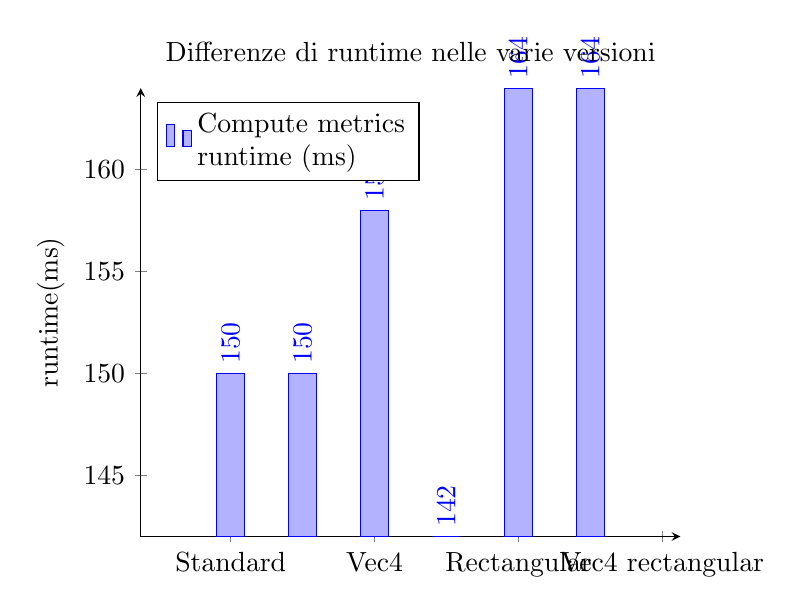
\begin{tikzpicture}
    \begin{axis}[ybar, title={Differenze di runtime nelle varie versioni}, symbolic x coords={
                Standard,
                Standard transpose,
                Vec4,
                Vec4 transpose,
                Rectangular,
                Vec4 rectangular},         
              legend pos = north west, axis y line=left, axis x line=bottom, nodes near coords, enlarge x limits=0.25, ylabel= runtime(ms), every node near coord/.append style={rotate=90, anchor=west}] 
            \addplot+ coordinates {(Standard, 150) (Standard transpose, 150) (Vec4, 158) (Vec4 transpose, 142) (Rectangular, 164) (Vec4 rectangular, 164)};
            \addlegendentry[align=left]{Compute metrics \\ runtime (ms)}; \end{axis} 
\end{tikzpicture}

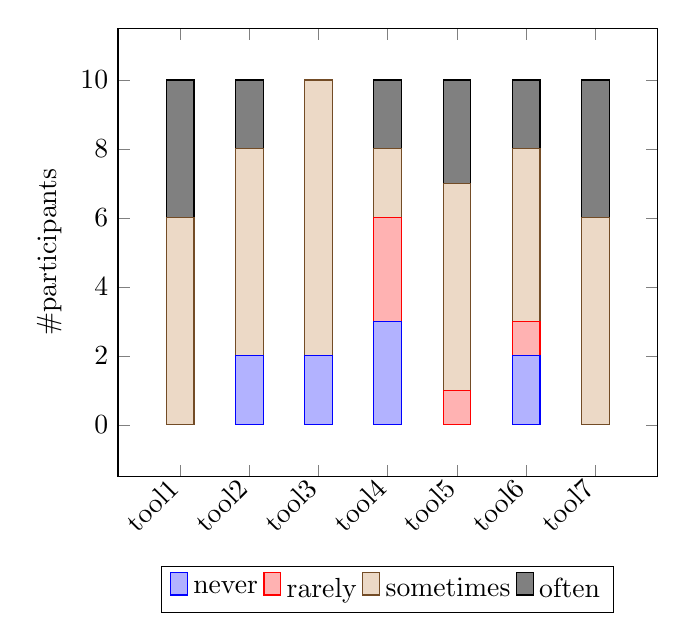
\begin{tikzpicture}
\begin{axis}[
ybar stacked,
enlargelimits=0.15,
legend style={at={(0.5,-0.20)},
anchor=north,legend columns=-1},
ylabel={\#participants},
symbolic x coords={tool1, tool2, tool3, tool4,
tool5, tool6, tool7},
xtick=data,
x tick label style={rotate=45,anchor=east},
]
\addplot+ [ybar] coordinates {(tool1,0) (tool2,2)
(tool3,2) (tool4,3) (tool5,0) (tool6,2) (tool7,0)};
\addplot+ [ybar] coordinates {(tool1,0) (tool2,0)
(tool3,0) (tool4,3) (tool5,1) (tool6,1) (tool7,0)};
\addplot+ [ybar] coordinates {(tool1,6) (tool2,6)
(tool3,8) (tool4,2) (tool5,6) (tool6,5) (tool7,6)};
\addplot+ [ybar] coordinates {(tool1,4) (tool2,2)
(tool3,0) (tool4,2) (tool5,3) (tool6,2) (tool7,4)};
\legend{never, rarely, sometimes, often}
\end{axis}
\end{tikzpicture}


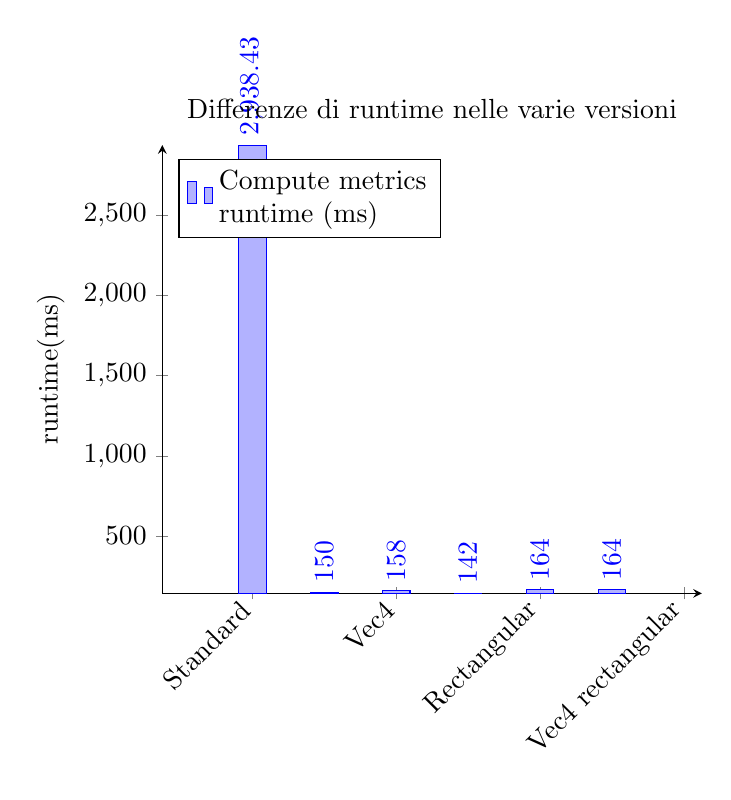
\begin{tikzpicture}
\begin{axis}[
ybar, 
title={Differenze di runtime nelle varie versioni}, 
symbolic x coords={
Standard,
Standard transpose,
Vec4,
Vec4 transpose,
Rectangular,
Vec4 rectangular},   
x tick label style={rotate=45,anchor=east},      
legend pos = north west, 
axis y line=left, 
axis x line=bottom, 
nodes near coords, 
enlarge x limits=0.25, 
ylabel= runtime(ms), 
every node near coord/.append style={
rotate=90, 
anchor=west}
] 
\addplot+ coordinates {(Standard, 2938.43) (Standard transpose, 150) (Vec4, 158) (Vec4 transpose, 142) (Rectangular, 164) (Vec4 rectangular, 164)};
\addlegendentry[align=left]{Compute metrics \\ runtime (ms)}; \end{axis} 
\end{tikzpicture} 


\end{document}